\begin{pr}$ $
\begin{enumerate}[(a)]
\item $\overline{m_1}=\min_{t\in T}\max_{s\in S}\pi_1(s, t)=\min(1, 2)=1$.\\
$\overline{m_2}=\min_{s\in S}\max_{t\in T}\pi_2(s, t)=\min(2, 1)=1$.\\
$\so$ by Folk theorem, the payoffs they could achieve in a Nash equilibrium is larger than or equal to $(\overline{m_1}, \overline{m_2})=(1, 1)$.\\
Therefore, the payoffs they could achieve in a Nash equilibrium is the colored region in the following graph:\\
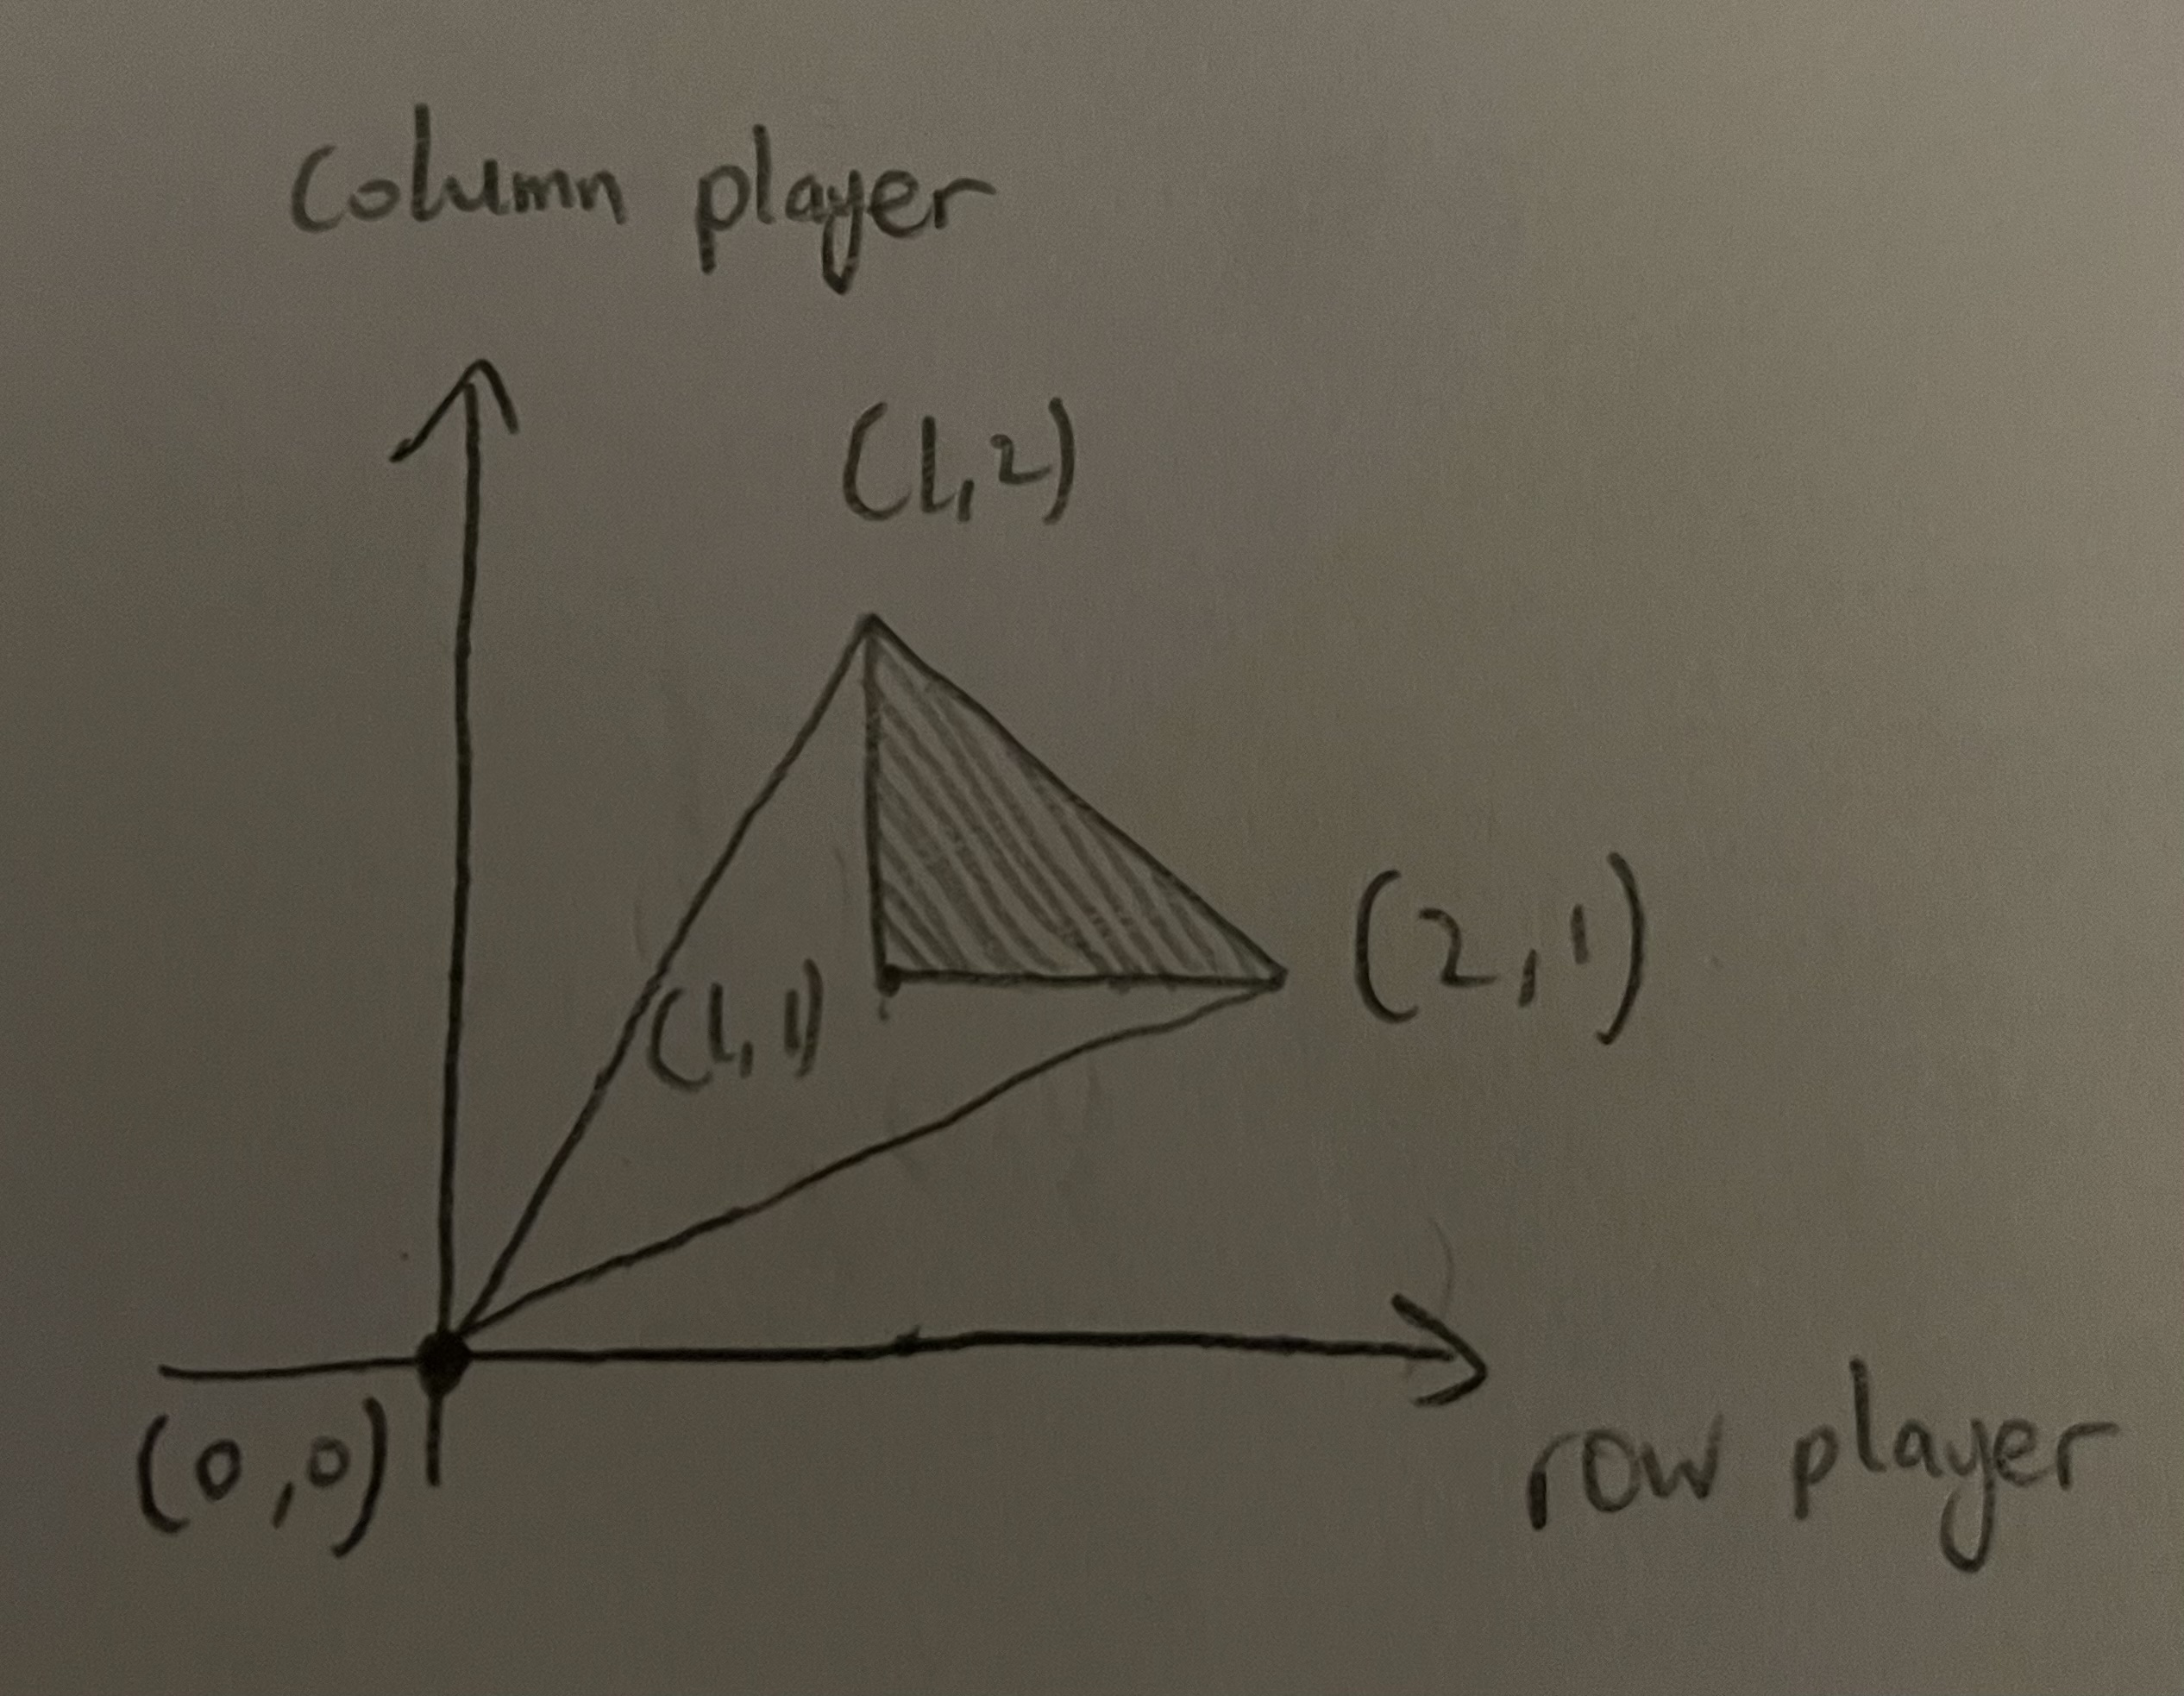
\includegraphics[width=15cm]{1a.JPG}
% picture
\item The upper one is the row player's strategy, while the bottom one is the columns player's strategy. The strategy is to play $(s_1, s_1), (s_1, s_1), (s_2, s_2)$ cyclically. Since if one of them change the strategy, their long-run average payoff will decrease to $1$, no one can change the strategy to achieve a better payoff. Therefore, the following strategy is a Nash equilibrium.\\
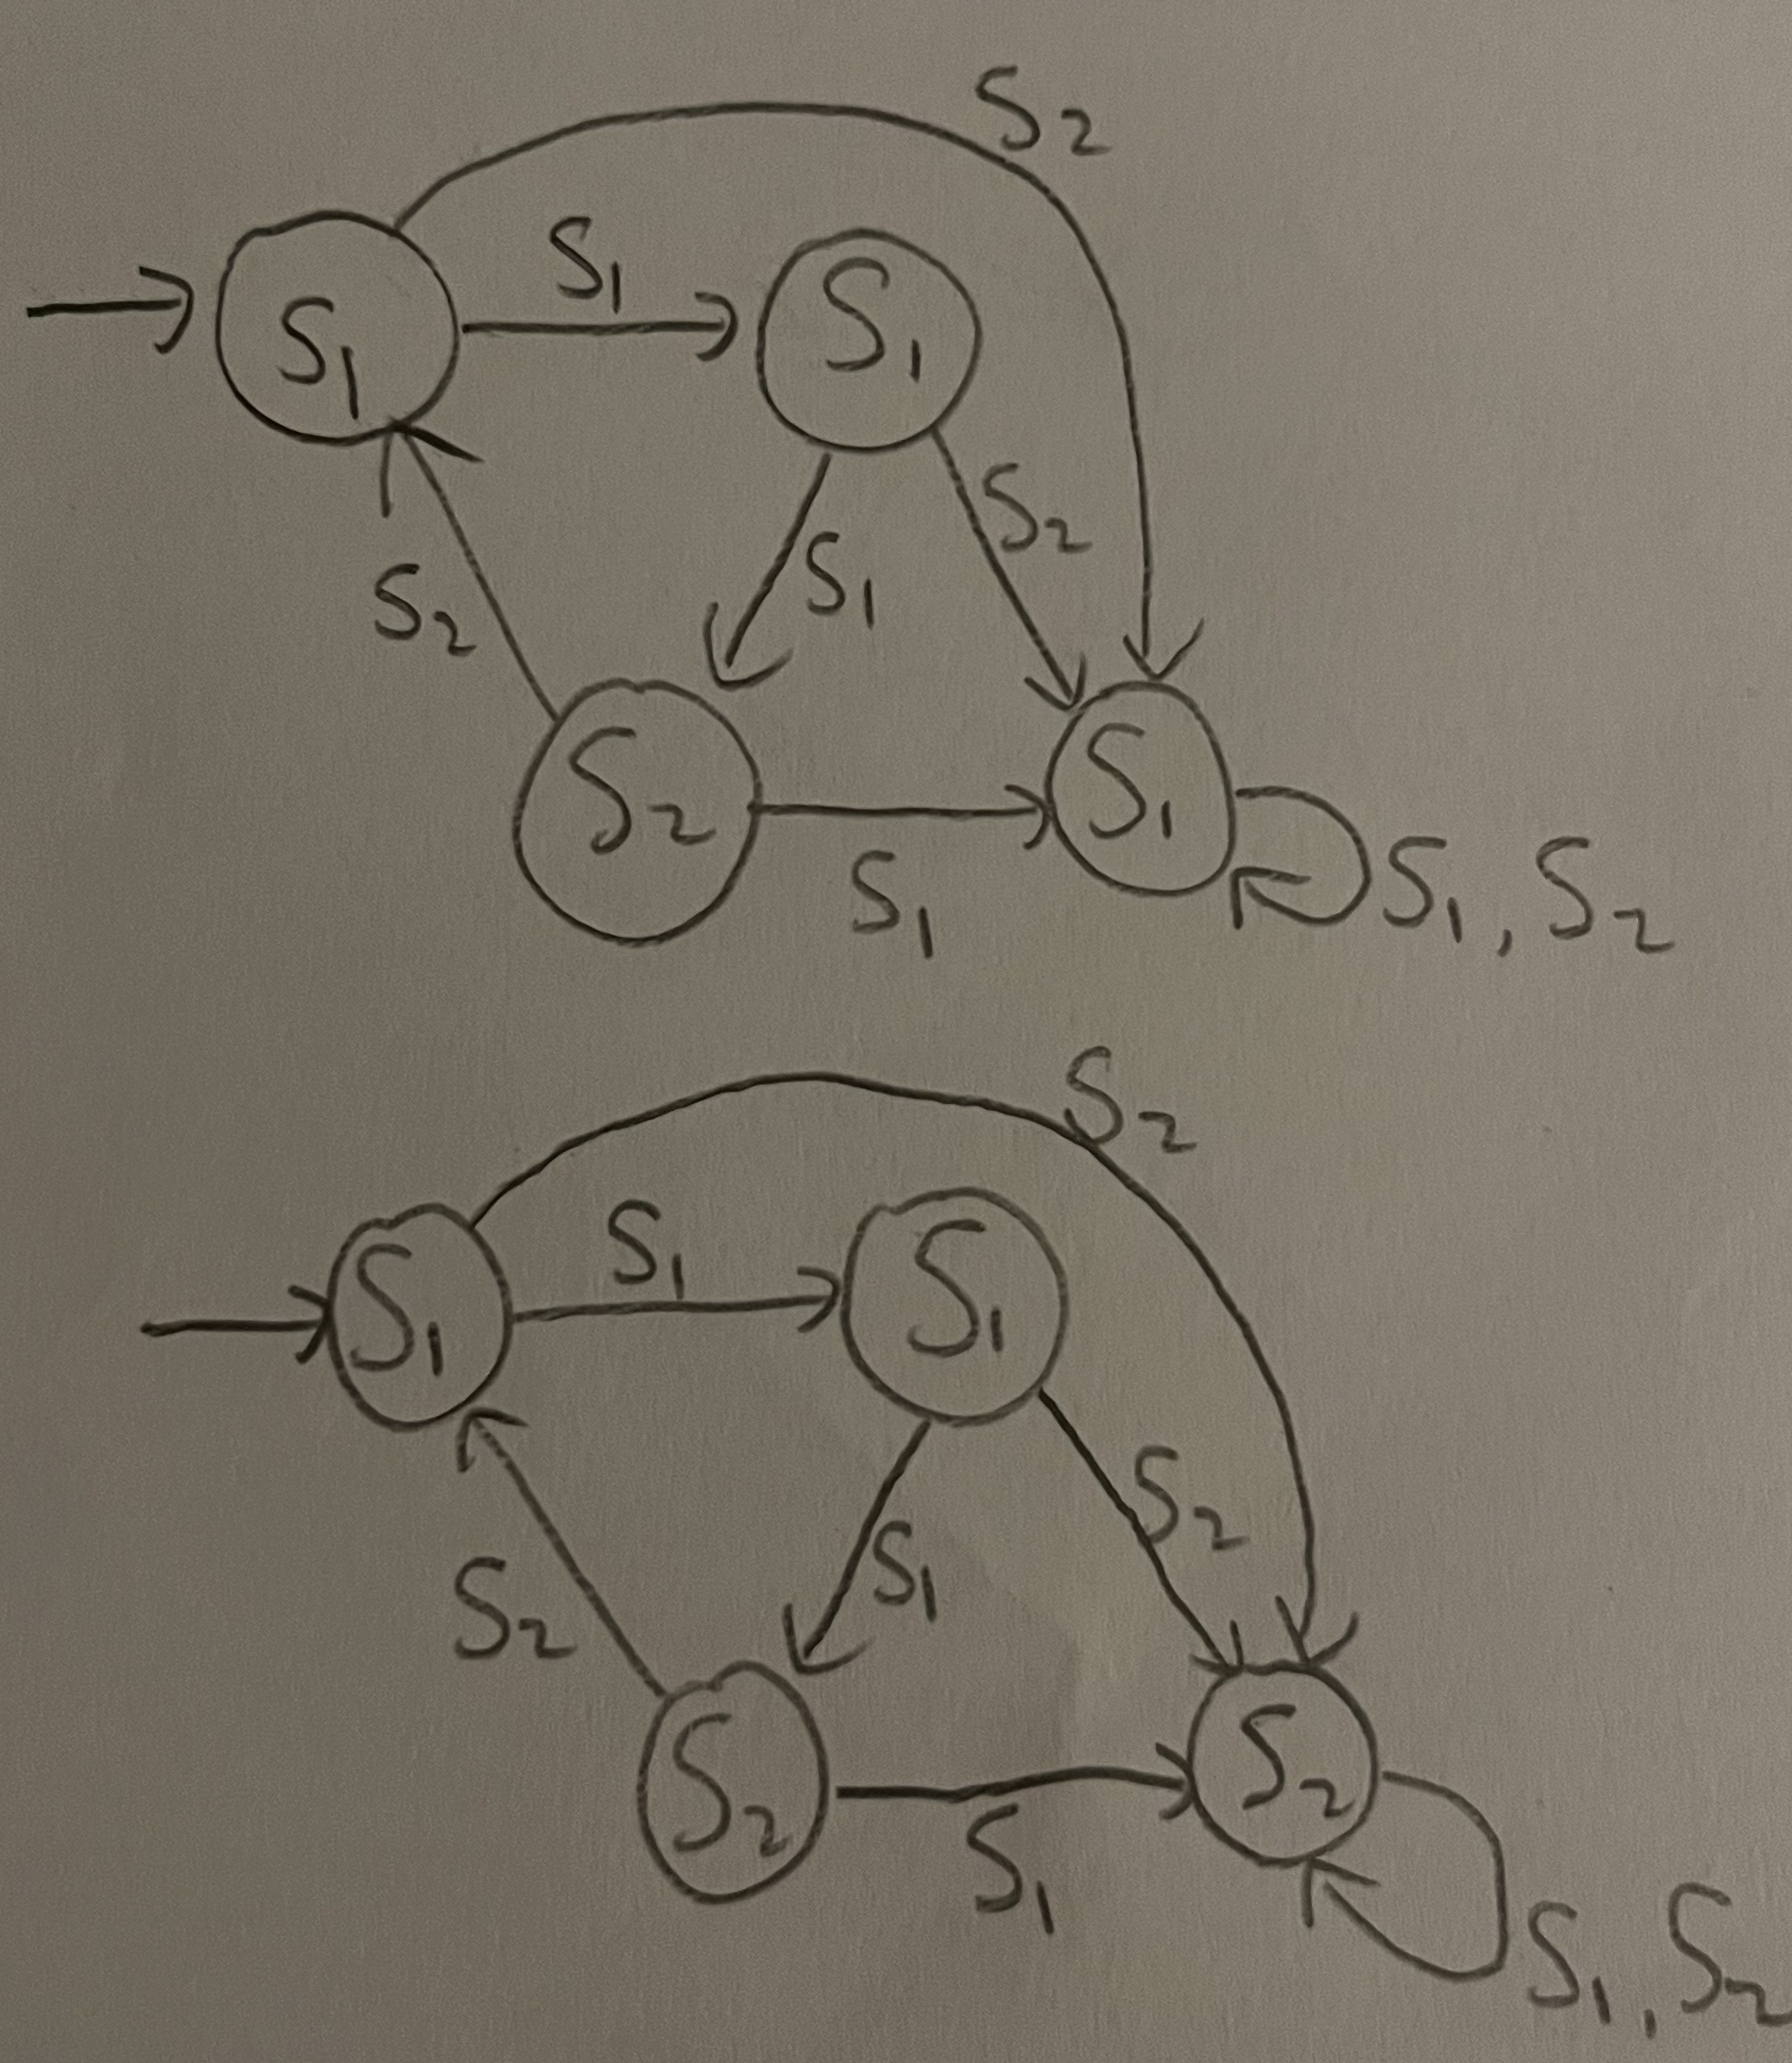
\includegraphics[width=15cm]{1b.JPG}
% picture
\item Suppose that $(p, 1-p)$ is the row player's mixed strategy.\\
$\underline{v_1}=\max_p\min_{t\in T}\E(\pi_1(s, t))=\max_p\min(2p, 1-p)=\frac23$, where $p=\frac13$.\\
Similarly, $\underline{v_2}=\frac23$.\\
$\so$ by Folk theorem, the payoffs they could achieve in a Nash equilibrium is larger than or equal to $(\frac23, \frac23)$.\\
Therefore, the payoffs they could achieve in a Nash equilibrium is the colored region in the following graph:\\
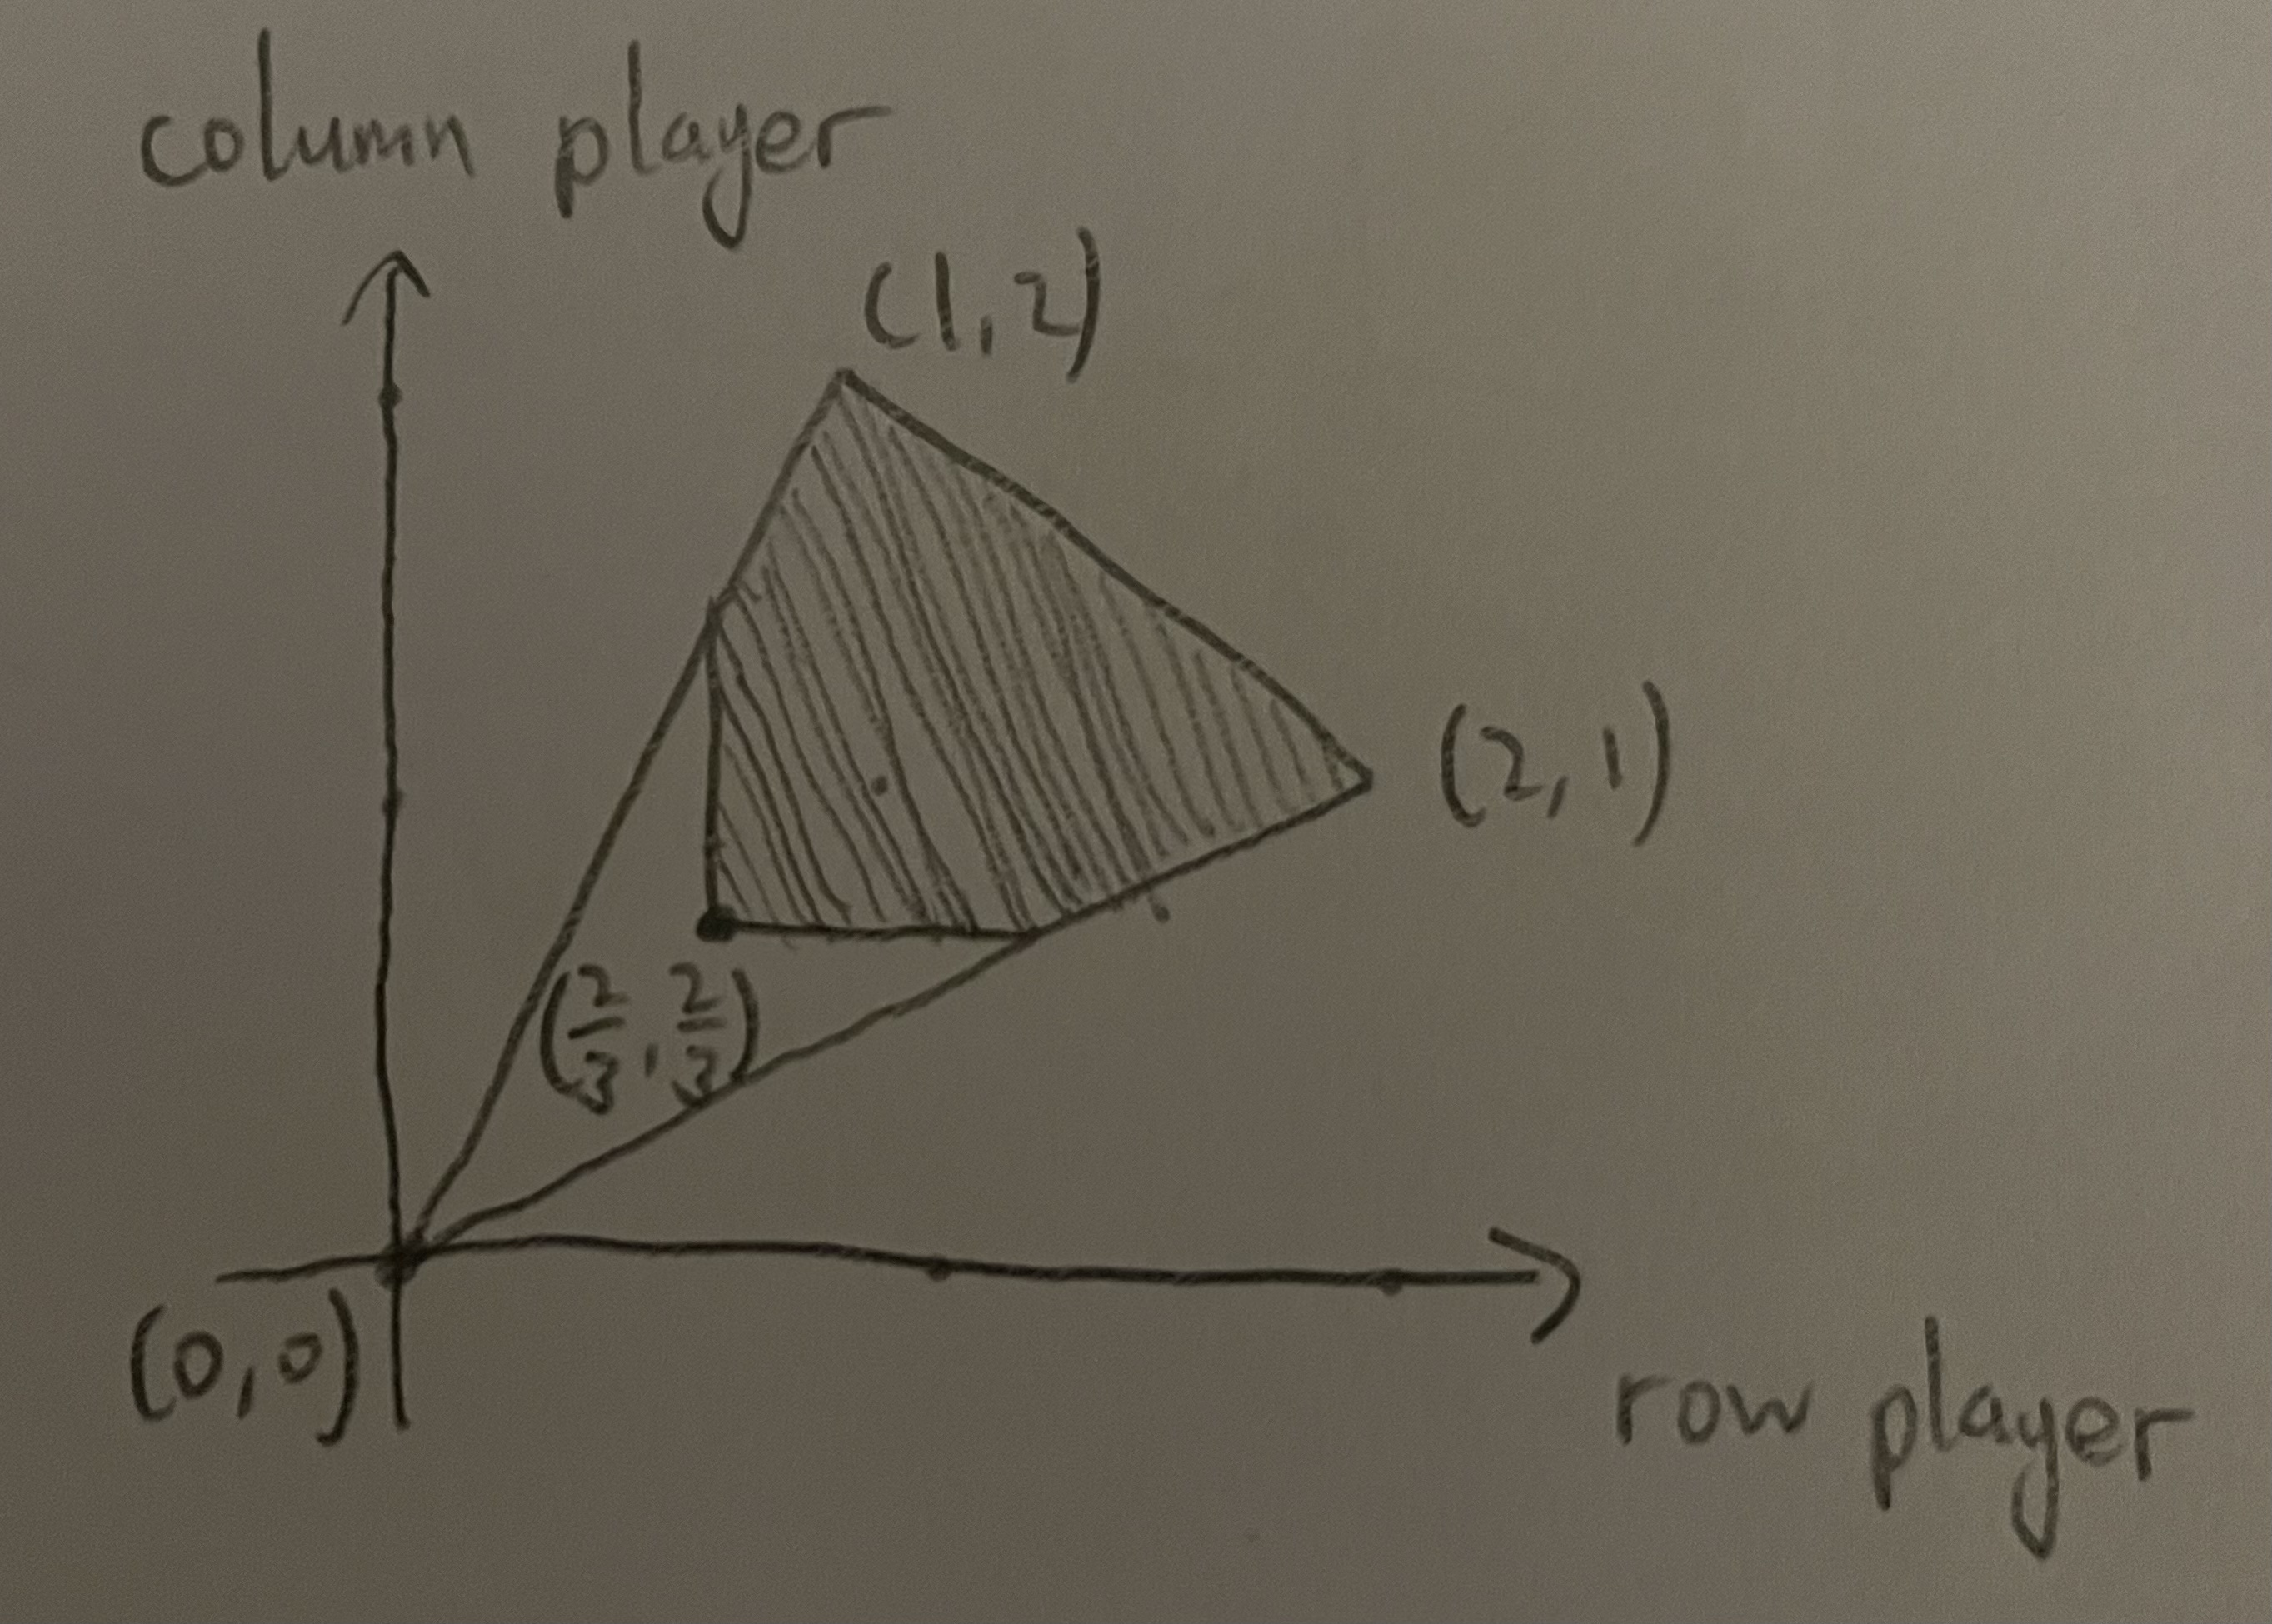
\includegraphics[width=15cm]{1c.JPG}
% picture
\end{enumerate}
\end{pr}
